\documentclass[12pt]{article}
\usepackage{amsmath}
\usepackage{amssymb}
\usepackage[letterpaper,top=1.35in,bottom=0.75in,left=0.75in,right=0.75in,centering]{geometry}
\usepackage{fancyhdr}
\usepackage{enumerate}
\usepackage{lastpage}
\usepackage{multicol}
\usepackage{graphicx}
\usepackage{vwcol}
\reversemarginpar
\usepackage{tikz}
\usetikzlibrary{calc, positioning, decorations.pathmorphing}


\pagestyle{fancy}
\cfoot{Page \thepage \ of \pageref{LastPage}}\rfoot{{\bf Total Points: 24}}
\lhead{\hspace*{2.2in}\underline{MATH 1560: Test 4}}

\newcommand{\points}[1]{\marginpar{\hspace{24pt}[#1]}}
\newcommand{\skipline}{\vspace{12pt}}
\renewcommand{\headrulewidth}{0in}
\headheight 20pt

\newcommand{\di}{\displaystyle}
\newcommand{\abs}[1]{\lvert #1\rvert}
\newcommand{\R}{\mathbb{R}}
\newcommand{\C}{\mathbb{C}}
\renewcommand{\P}{\mathcal{P}}
\DeclareMathOperator{\nul}{null}
\DeclareMathOperator{\range}{range}
\DeclareMathOperator{\spn}{span}
\newcommand{\len}[1]{\lVert #1\rVert}
\newcommand{\Q}{\mathbb{Q}}
\newcommand{\N}{\mathbb{N}}
\renewcommand{\L}{\mathcal{L}}
\newcommand{\dotp}{\boldsymbol{\cdot}}
\newenvironment{amatrix}[1]{%
  \left[\begin{array}{@{}*{#1}{c}|c@{}}
}{%
  \end{array}\right]
}
\newcommand{\bam}{\begin{amatrix}}
\newcommand{\eam}{\end{amatrix}}
\newcommand{\bbm}{\begin{bmatrix}}
\newcommand{\ebm}{\end{bmatrix}}

\begin{document}


 \begin{enumerate}
 \item  Find and classify the critical points of \points{5}
 \[
 f(x) = x^3(1-x)^2.
 \]
 
 \medskip
 
 \textbf{Solution:} We first compute the derivative of $f$. If we take the function as written, using the product and chain rules, and then taking out common factors, we get
 \[
 f'(x) = 3x^2(1-x)^2+x^3(2(1-x)(-1))=x^2(1-x)(3(1-x)-2x) = x^2(1-x)(3-5x).
 \]
 Alternatively, we could first re-write $f(x)$ by expanding the square:
 \[
 f(x) = x^3(1-2x+x^2) = x^3-2x^4+x^5, \text{ so } f'(x) = 3x^2-8x^3+5x^4.
 \]
 Taking out the common factor of $x^2$ and then factoring the resulting quadratic gives the same result as above.
 
 From the factored expression for $f'(x)$, we see that $f'(x)=0$ when $x=0$, $x=3/5$, and $x=1$. Each of these is a critical number, since the domain of $f$ is $\R$. To classify, we construct the sign diagram for $f'$ and use the First Derivative Test.
 \begin{center}
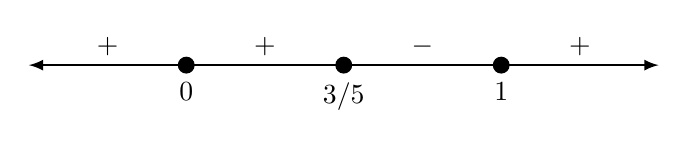
\begin{tikzpicture}[>=latex]
  \draw [thick, <->] (-4,0) -- (4,0);
  \draw [fill] (-2,0) circle [radius =.1];
  \draw [fill] (0,0) circle [radius =.1];
  \draw [fill] (2,0) circle [radius =.1];
  \node at (-3,0) [above] {$+$};
  \node at (-1,0) [above] {$+$};
  \node at (1,0) [above] {$-$};
  \node at (3,0) [above] {$+$};
  \node at (-2,-0.1) [below] {$0$};
  \node at (0,-0.1) [below] {$3/5$};
  \node at (2,-0.1) [below] {$1$};
  \end{tikzpicture}
\end{center}
 Since the derivative switches from positive to negative at $3/5$, the point $(3/5, f(3/5))$ is a local maximum. Since the derivative switches from negative to positive at $1$, the point $(1,0)$ is a local minimum. Since the derivative does not change sign at $x=0$, the point $(0,0)$ is neither a local maximum nor a local minimum.
 
 \newpage
 
 \item A street light is at the top of a 18 foot tall pole. A 6 foot tall circus bear (who has learned to walk upright) walks away from the pole with a speed of 4 ft/sec along a straight path. 
\begin{enumerate}
\item Draw a diagram of the situation. \points{1}
\item At what rate is the length of her shadow increasing when she is 30 feet from the pole?\points{2}
\item How fast is the tip of her shadow moving when she is 30 feet from the pole? \points{2}

\medskip

\begin{multicols}{2}
\textbf{Solution:} We let $x$ denote the distance from the pole to the bear, and we let $y$ denote the length of the shadow, as indicated in the diagram on the right. Using similar triangles, we obtain the relationship
\[
\frac{y}{6}=\frac{x+y}{18},
\]

\begin{center}
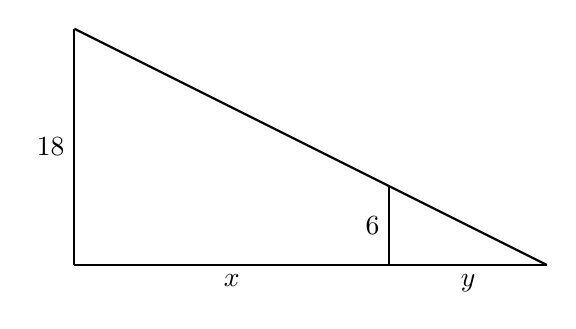
\begin{tikzpicture}[>=latex]
\draw [thick] (-3,3) -- (-3,0);
\draw [thick] (-3,0) -- (3,0);
\draw [thick] (-3,3) -- (3,0);
\draw [thick] (1,0) -- (1,1);
\node at (-3,1.5) [left] {$18$};
\node at (1,0.5) [left] {$6$};
\node at (-1,0) [below] {$x$};
\node at (2,0) [below] {$y$};
\end{tikzpicture}
\end{center}
\end{multicols}
since the sides of the small triangle must be proportional to those of the large triangle.
Simplifying the equation above, we obtain $18y=6x+6y$, so $12y=6x$, or $y=\frac{1}{2}x$. Taking the derivative of both sides of this equation with respect to $t$, we find
\[
\frac{dy}{dt}=\frac{1}{2}\frac{dx}{dt}.
\]
We identify that $\frac{dx}{dt}=4$ ft/s is the speed at which the bear is walking, and $\frac{dy}{dt} = \frac{1}{2}(4)=2$ is the rate at which the length of the shadow is increasing. Thus, the length of the shadow is increasing at a rate of 2 ft/s.

To determine the speed at which the tip of the shadow is moving, we note that this is the same as the rate at which the distance from the pole to the tip of the shadow is increasing. Since this distance is $x+y$, we find that the tip of the shadow is moving at a speed of
\[
\frac{d}{dt}(x+y) = \frac{dx}{dt}+\frac{dy}{dt} = 4 \text{ ft/s} + 2 \text{ ft/s} = 6 \text{ ft/s}.
\]
\end{enumerate} 
 \newpage
 
 \item Let $f(x) = x^4-4x^3$.
 \begin{enumerate}
 \item Determine a sign diagram for $f(x)$. \points{2} State the domain of $f$, and list any intercepts or asymptotes.
 
 Since $f(x)=x^3(x-4)$, we have $x$-intercepts $(0,0)$ (also the $y$-intercept) and $(4,0)$. The domain of $f$ is $\R$ (or equivalently, $(-\infty,\infty)$). There are no asymptotes. The sign diagram is given by
 \begin{center}
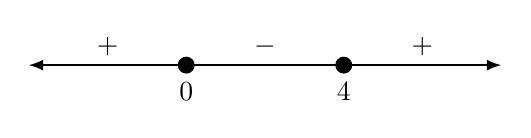
\begin{tikzpicture}[>=latex]
  \draw [thick, <->] (-3,0) -- (3,0);
  \draw [fill] (-1,0) circle [radius =.1];
  \draw [fill] (1,0) circle [radius =.1];
  \node at (-2,0) [above] {$+$};
  \node at (0,0) [above] {$-$};
  \node at (2,0) [above] {$+$};
  \node at (-1,-0.1) [below] {$0$};
  \node at (1,-0.1) [below] {$4$};
  \end{tikzpicture}
\end{center}
 \item Determine a sign diagram for $f'(x)$. \points{3} State the intervals on which $f$ is increasing or decreasing.
 
 \medskip
 
 From $f(x)=x^4-4x^3$, we find
 \[
 f'(x) = 4x^3-12x^2 = 4x^2(x-3).
 \]
 The sign diagram is given by
  \begin{center}
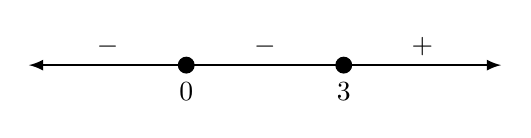
\begin{tikzpicture}[>=latex]
  \draw [thick, <->] (-3,0) -- (3,0);
  \draw [fill] (-1,0) circle [radius =.1];
  \draw [fill] (1,0) circle [radius =.1];
  \node at (-2,0) [above] {$-$};
  \node at (0,0) [above] {$-$};
  \node at (2,0) [above] {$+$};
  \node at (-1,-0.1) [below] {$0$};
  \node at (1,-0.1) [below] {$3$};
  \end{tikzpicture}
\end{center}
From the sign diagram, we see that $f$ is increasing on $(3,\infty)$  and decreasing on $(-\infty,3)$.

 \item Determine a sign diagram for $f''(x)$.\points{3} State the intervals on which the graph of $f$ is concave up or concave down.
 
 \medskip
 
Starting from $f'(x) = 4x^3-12x^2$, we find
\[
f''(x) = 12x^2-24x=12x(x-2).
\]
The sign diagram is given by
 \begin{center}
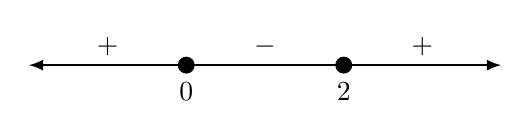
\begin{tikzpicture}[>=latex]
  \draw [thick, <->] (-3,0) -- (3,0);
  \draw [fill] (-1,0) circle [radius =.1];
  \draw [fill] (1,0) circle [radius =.1];
  \node at (-2,0) [above] {$+$};
  \node at (0,0) [above] {$-$};
  \node at (2,0) [above] {$+$};
  \node at (-1,-0.1) [below] {$0$};
  \node at (1,-0.1) [below] {$2$};
  \end{tikzpicture}
\end{center}
From the sign diagram, we see that the graph of $f$ is concave up on $(-\infty,0)\cup (0,\infty)$, and concave down on $(0,2)$.

 \item Sketch the graph of $f$.\points{2} Be sure to label all intercepts, critical points, and inflection points.
 
 \medskip
 
 From our work above, we can see that the point $(0,0)$ is an intercept, a critical point (corresponding to a horizontal tangent that is neither a maximum nor a minimum), and an inflection point. There is also a local minimum at $(3,-27)$, an inflection point at $(2,-16)$, and another intercept at $(4,0)$. Plotting these points, and using the sign diagrams for $f'$ and $f''$ to get the correct behaviour between them, we obtain the following graph (the $y$-axis has been rescaled to fit things on the page):
 \begin{center}
 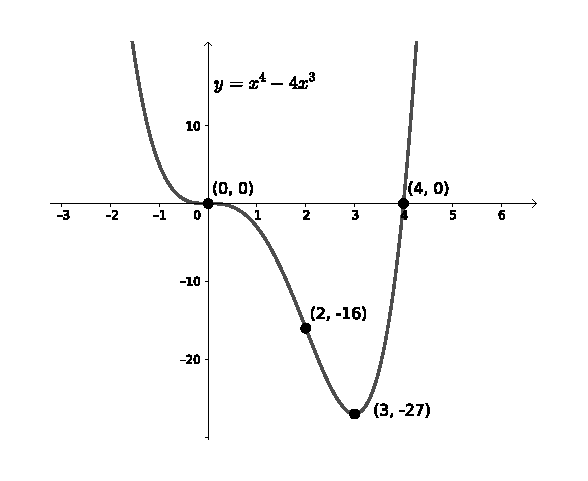
\includegraphics[width=4in]{TT4-fig2}
 \end{center}
 \end{enumerate}
 \newpage

\item \textbf{Extra group question!}

\medskip

Consider the function $f(x)=\dfrac{x}{x^2+4}$, for $x\in (-\infty, \infty)$. Even though you are not given a closed interval, this function does have an absolute maximum and absolute minimum.

\medskip

Find these values, and justify your answer. \points{4}

\bigskip

\textit{Suggestion:} You might find it helpful to consider the graph, and/or the behaviour of $f(x)$ as $x\to \pm \infty$. Since there are no endpoints, any global extrema must occur at local extrema. 

\bigskip

\textbf{Solution:} We note that $y=0$ is a horizontal asymptote for $y=f(x)$, and that there are no vertical asymptotes.

Since the graph tends towards zero for large values of $x$ (both positive and negative), any extreme values must be local extreme values. To find the local extrema, we look for critical numbers:

\[
f'(x) = \frac{1(x^2+4)-x(2x)}{(x^2+4)^2} = \frac{4-x^2}{(x^2+4)^2} = \frac{(2-x)(2+x)}{(x^2+4)^2}.
\]
We have $f'(x)=0$ when $x=\pm 2$; from the sign diagram 
\begin{center}
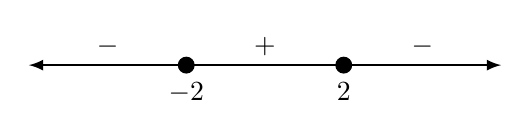
\begin{tikzpicture}[>=latex]
  \draw [thick, <->] (-3,0) -- (3,0);
  \draw [fill] (-1,0) circle [radius =.1];
  \draw [fill] (1,0) circle [radius =.1];
  \node at (-2,0) [above] {$-$};
  \node at (0,0) [above] {$+$};
  \node at (2,0) [above] {$-$};
  \node at (-1,-0.1) [below] {$-2$};
  \node at (1,-0.1) [below] {$2$};
  \end{tikzpicture}
\end{center}
we see that $(2,1/4)$ is a local maximum, and $(-2,-1/4)$ is a local minimum, and these must in fact be the global maximum and minimum. We can confirm this by considering the graph:
\begin{center}
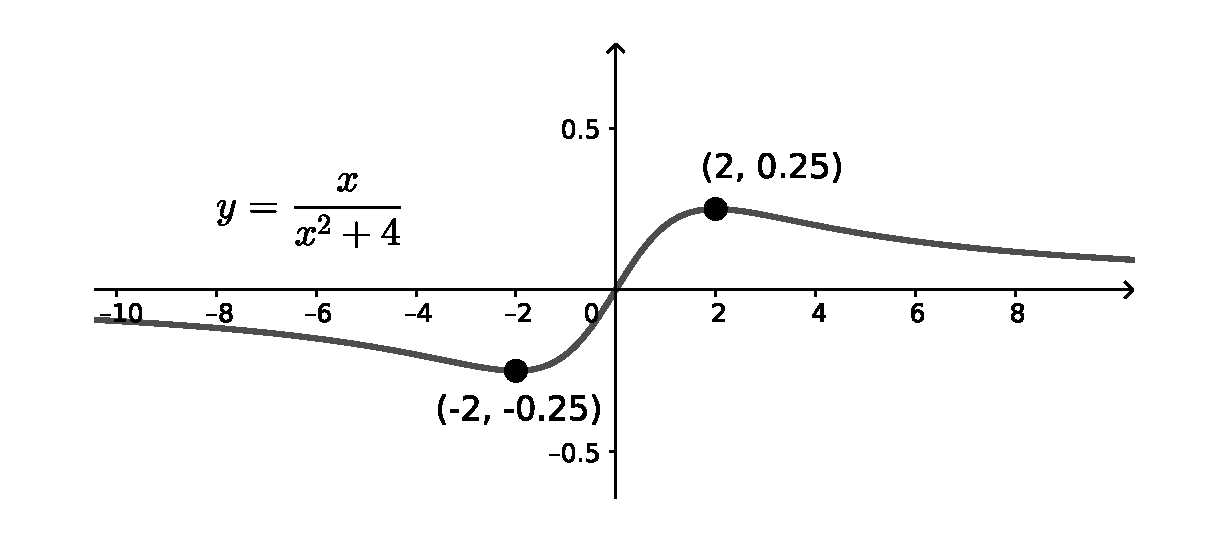
\includegraphics[width=4in]{TT4-fig3}
\end{center}


\end{enumerate}
\end{document}